%%==================================================================%%
%% Author : Tejedo Gonz�lez, Daniel                                 %%
%%          S�nchez Barreiro, Pablo                                 %%
%% Version: 1.0, 27/11/2012                                         %%                   
%% Version: 2.0, 09/02/2013                                         %%                   
%%                                                                  %%
%% Memoria del Proyecto Fin de Carrera                              %%
%% Gram�tica,  archivo raiz                                         %%
%%==================================================================%%

\chapterheader{Creaci�n de la gram�tica}{Creaci�n de la gram�tica}
\label{chap:gramatica}

Una vez definida la sintaxis abstracta de nuestro lenguaje, el siguiente paso es definir su sintaxis concreta, que en nuestro caso se trata de una sintaxis textual. Este cap�tulo describe el proceso de desarrollo de una gram�tica que permita definir dicha sintaxis textual.

\chaptertoc

\section{Captura de requisitos}
\label{sec:gram:requisitos}
%%==================================================================%%
%% Author : Tejedo Gonz�lez, Daniel                                 %%
%%          S�nchez Barreiro, Pablo                                 %%
%% Version: 1.0, 25/11/2012                                         %%
%% Version: 2.0, 06/02/2013                                         %%
%%                                                                  %%
%% Memoria del Proyecto Fin de Carrera                              %%
%% Sintaxis abstracta, requisitos                                   %%
%%==================================================================%%

El primer paso para desarrollar nuestro lenguaje era conocer qu� aspecto deb�a tener nuestro lenguaje y qu� restricciones deb�a satisfacer. Es decir, en primer lugar debemos realizar un proceso que podemos denominar de captura de requisitos para poder comprender qu� es lo que tiene que hacer exactamente el lenguaje que se pretende crear.

Concretamente nuestro lenguaje hab�a sido pr�cticamente definido por el profesor Pablo S�nchez, del Departamento de Matem�ticas, Estad�stica y Computaci�n de la Universidad de Cantabria, mediante notaci�n BNF. Las ideas subyacentes a dicho lenguaje son las que se describen a continuaci�n. Como apoyo a la descripci�n, la Figura~\ref{fig:constraintBNF} muestra la sintaxis del lenguaje en notaci�n EBNF.

\begin{figure}[!tb]
    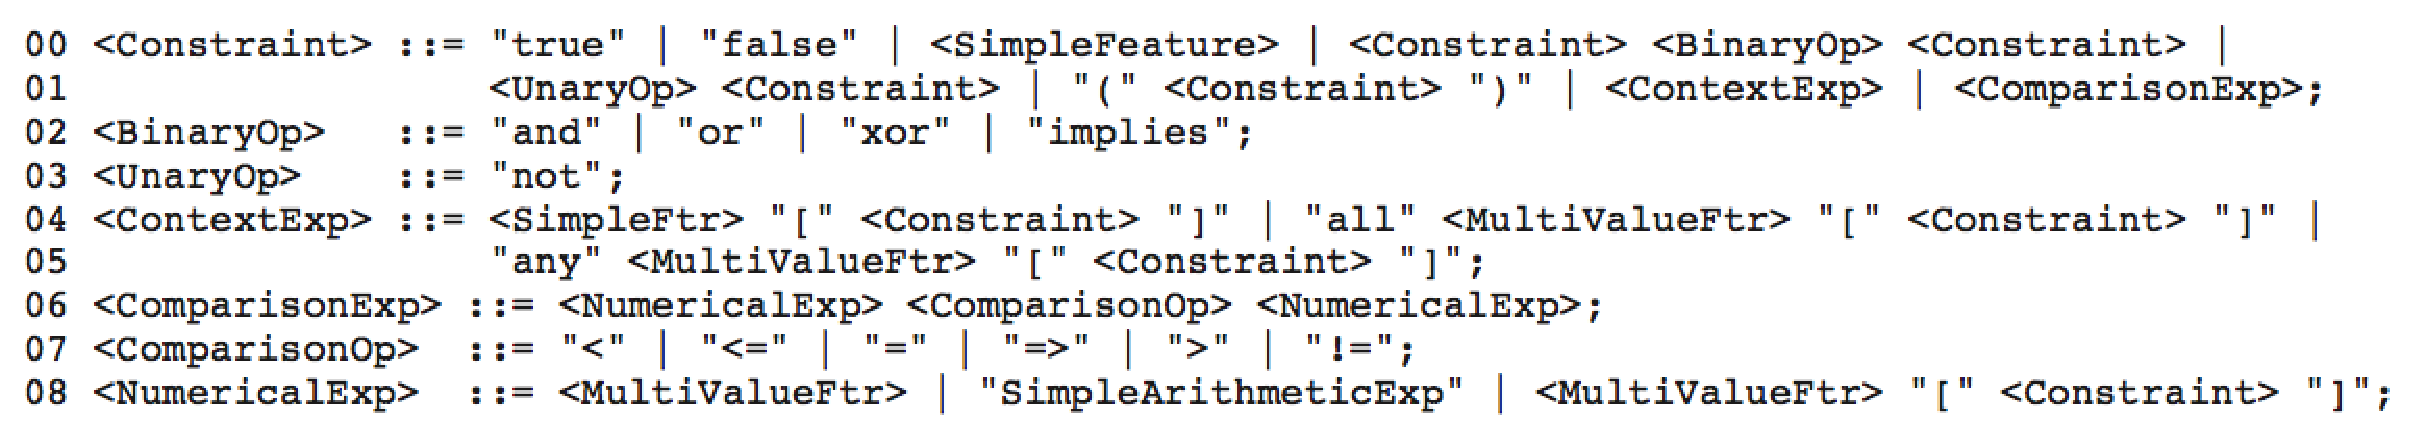
\includegraphics[scale=0.3]{metamodelo/constraintBNF.eps}
    \caption{Lenguaje de restricciones en notaci�n EBNF}
    \label{fig:constraintBNF}
\end{figure}

Una \emph{restricci�n} es una expresi�n l�gica que se puede evaluar a verdadero o falso. Una restricci�n puede ser simplemente un literal, es decir, $true$ o $false$, que se evaluar� a verdadero y falso respectivamente. Una restricci�n tambi�n puede ser una caracter�stica simple, es decir, una caracter�stica que puede aparecer en las configuraciones como m�ximo una vez. Una caracter�stica simple se eval�a a verdadero si ha sido seleccionado, y a falso en caso contrario.

Las caracter�sticas clonables son aquellas que pueden ser seleccionadas m�s de una vez en las configuraciones que construyamos sobre nuestro �rbol de caracter�sticas. Una caracter�stica clonable se eval�an como un n�mero entero positivo, incluido el cero. Ese n�mero representa el n�mero de clones que la caracter�stica posee dentro de una configuraci�n, o dicho de otro modo, el n�mero de veces que ha sido seleccionada. El hecho de que se eval�en como si fueran n�meros permite la inclusi�n de operaciones de comparaci�n que permitan definir restricciones comparativas entre distintas caracter�sticas clonables. Las operaciones de comparaci�n que se han de implementar son las siguientes: $<$,$<$=,$>$,$>$=,=,!= . Adem�s, tambi�n se puede utilizar el valor de las caracter�sticas clonables para implementar operaciones aritm�ticas b�sicas, tales como la suma, la resta, la multiplicaci�n y la divisi�n. Estas expresiones a su vez se pueden utilizar como subexpresiones, u operandos, dentro de las operaciones de comparaci�n. Las expresiones de comparaci�n se eval�an a verdadero o falso, y tambi�n pueden ser usadas como subexpresiones para crear expresi�n l�gica m�s compleja. 

Tal y como muestra la Figura~\ref{fig:constraintBNF}, una restricci�n tambi�n puede especificar un contexto concreto en el que poder evaluarla. Esto puede hacerse de varias maneras. Se puede especificar un contexto para una restricci�n poni�ndola entre corchetes y especificando el nombre de una caracter�stica al principio de la expresi�n. La caracter�stica usada como contexto puede ser tanto simple como m�ltiple. En el primer caso, la restricci�n s�lo ser� evaluada en el sub�rbol de la configuraci�n cuya ra�z sea la caracter�stica especificada.

En el segundo caso entran en juego los operadores $all$ (para todo) y $any$ (existe). La operaci�n $all$ solo se evaluar� a verdadero si la restricci�n entre corchetes se cumple para todas las selecciones de la caracter�stica clonable. En caso contrario, la operaci�n se evaluar� a falso. La operaci�n $any$ se evaluar� a verdadero si la restricci�n entre corchetes se cumple al menos una vez para todas las selecciones de la caracter�stica. Si la restricci�n no se cumple para ninguna de las selecciones, la operaci�n $any$ se evaluar� a falso. 

Merece la pena se�alar que una caracter�stica puede ser considera simple en un contexto determinado y clonable o m�ltiple en otro. Por ejemplo, la caracter�stica $LightMng$ es clonable en el contexto de $RoomFacilities$, pero simple en el contexto de $GeneralFacilities$. Debido a eso la caracter�stica $LightMng$ no puede ser utilizada a la ligera sin especificar el contexto en el que est� ubicada, pues podr�a provocar un resultado no esperado o err�neo.

En la restricci�n $any Room[RoomFacilities[LightMng]]$ se pueden apreciar los dos diferentes usos para la operaci�n de contexto. Los corchetes externos indican a la operaci�n any que hay que aplicar la restricci�n a todas las habitaciones. Los corchetes internos indican que la caracter�stica $LightMng$ a la que se est� haciendo referencia es la hija de $RoomFacilities$ y no cualquier otra.

%%==================================================================%%
%% NOTA(Pablo): Aqu� traduce la secci�n III del art�culo que te
%%              env�o adjunto. Si te hacen falta las fuentes del
%%              art�culo, me las pides.
%%
%%              Traduce primero del ingl�s y luego lo repasas y lo
%%              reescribes para que suene a castellano
%% 
%%              Si en la secci�n III no aparecen las razones por 
%%              las cuales una caracter�stica es clonable, buscar 
%%              en qu� parte del art�culo aparecen y explicarlo

%%==================================================================%%

Adem�s nuestro lenguaje deb�a permitir vincular un modelo de caracter�sticas sobre el cual se definir�n un conjunto de restricciones externas. Este modelo se utilizar�, por ejemplo, para comprobar que los s�mbolos que aparecen como nombres de caracter�sticas en las restricciones se refieren a caracter�sticas que realmente existen en el �rbol de caracter�sticas. Por ejemplo, una restricci�n del tipo $AdvancedHeating => Heating$ carecer�a de sentido si algunas de las caracter�sticas $AdvancedHeating$ o $Heating$ no apareciesen en el �rbol de caracter�sticas sobre el cual estamos definiendo restricciones.

%%======================================================================================%%
%% NOTA(Pablo): Esto posiblemente sobre al introducir la traducci�n de la Secci�n III.
%%              Si es as�, eliminarla.
%%              Si los conceptos de restricci�n con contexto y operaci�n cuantificada
%%              no apareciesen, meter esta clasificaci�n pero resumida
%%======================================================================================%%
%%
%% De entre todos esos requisitos b�sicos, es necesario entrar en detalle en el n�mero 3
%% y enumerar la lista de operaciones que pueden ser definidas por nuestro lenguaje. Se
%% pueden clasificar en los siguientes tipos: \\
%%
%% - L�gicas: Son operaciones cuyos operandos han de ser caracter�sticas sin
%%   cardinalidad (tambi�n llamadas caracter�sticas simples), y que se evaluan a
%%   verdadero o falso. Entre las operaciones l�gicas encontramos las cl�sicas not,
%%   and, or, xor e implica.
%%
%% - Num�ricas: Sus operandos han de ser caracter�sticas con cardinalidad (tambi�n
%%   llamadas caracter�sticas m�ltiples) o simplemente n�meros. Su resultado se evalua
%%   con un valor num�rico. Las operaciones num�ricas a implementar son la suma, resta,
%%   multiplicaci�n y divisi�n.
%%
%% - Comparativas: Sus operandos han de ser caracter�sticas m�ltiples o simplemente n�meros,
%%   pero su resultado se evalua con un valor booleano. Las operaciones de comparaci�n a
%%   implementar son igual que, mayor que, menor que, distinto que, mayor o igual que y menor
%%   o igual que.
%%
%% - Operaci�n de contexto: Operaci�n que permite hacer referencia a una caracter�stica
%%   hija de otra caracter�stica. Esta operaci�n tiene sentido para seleccionar
%%   caracter�sticas cuyo nombre pueda estar repetido pero que tengan contextos diferentes.
%%   Por ejemplo, en el modelo de caracter�sticas SmartHome de la figura \ref{figsmarthome}
%%   podemos observar que la caracter�stica HeaterMng est� presente en muchos contextos
%%   diferentes. Esta operaci�n es necesaria para poder saber con seguridad a cual de esos
%%   contextos estamos aplicando la restricci�n.
%%
%% - Operaci�n de selecci�n: Operaci�n que corresponde a los operadores l�gicos cl�sicos
%%   "para todo" o "existe", y que tiene la misma funcionalidad. Evalua si una restricci�n
%%   se cumple para todos los casos en que puede existir  o si se cumple en alguno de los
%%   casos. Por ejemplo, en el modelo de la figura \ref{figsmarthome} se podr�a evaluar una
%%   restricci�n para cada una de las habitaciones que hayan sido definidas, y saber si se
%%  cumple en todas, en alguna o en ninguna.
%%
%%======================================================================================%%

Utilizando esta informaci�n como base, procedimos a crear el correspondiente metamodelo en Ecore para nuestro lenguaje.




\section{Dise�o de la gramatica}
\label{sec:gram:design}
%%==================================================================%%
%% Author : Tejedo Gonz�lez, Daniel                                 %%
%%          S�nchez Barreiro, Pablo                                 %%
%% Version: 1.0, 27/11/2012                                         %%                   %%                                                                  %%
%% Memoria del Proyecto Fin de Carrera                              %%
%% Gram�tica,  dise�o                                       %%
%%==================================================================%%

Una vez han sido definidas las caracter�sticas que queremos que nuestra sintaxis textual posea, el siguiente paso es dise�ar una gram�tica que se ajuste a ellas. 

La parte m�s trivial e inmediata del dise�o de la gram�tica es la concerniente a la implementaci�n de las operaciones, pues las producciones necesarias simplemente requieren la inclusi�n de los operandos involucrados y los caracteres que deseemos que definan la operaci�n. La figura \ref{figopers} muestra la implementaci�n de estas operaciones. 

\begin{figure}[t]
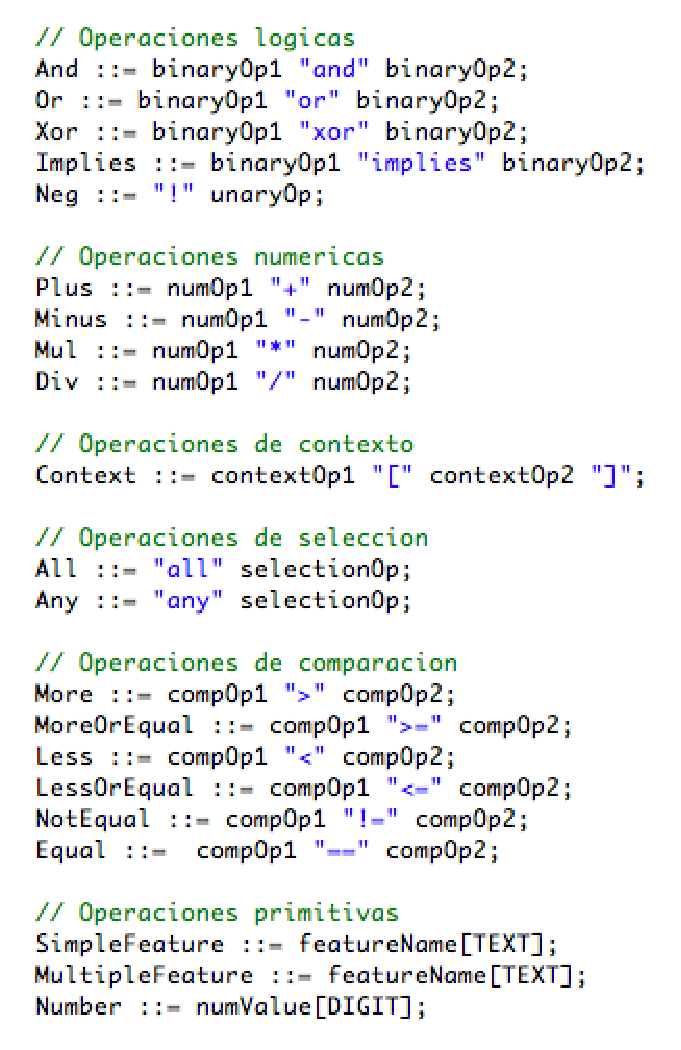
\includegraphics[scale=0.7]{gramatica/operaciones.eps}
\caption{Implementaci�n de las operaciones de nuestro editor com EMFText}
\label{figopers}
\end{figure}

S� que cabe comentar con respecto a las operaciones las �ltimas l�neas, que muestran la asignaci�n de valor a las hojas de nuestros �rboles parseados. En esas l�neas estamos indicando que los atributos de las instancias de clase Number van a ser n�meros, y que los atributos de las instancias de las clases SimpleFeature y MultipleFeature van a ser palabras.

La parte m�s complicada corresponde a la implementaci�n del inicio de la gram�tica y de las producciones que conducen a la misma. Pero antes de mostrar la figura con esta parte de la gram�tica conviene explicar el problema que llev� a realizar los cambios en el metamodelo mencionados en el cap�tulo anterior. Este problema surgi� a la hora de implementar las operaciones con prioridad, es decir, la inclusi�n de los par�ntesis.

El inconveniente es que el tipo de gram�tica LL que implementa EMFText hac�a imposible tomar una decisi�n sobre hacia qu� elemento seguir parseando en caso de encontrarnos con un par�ntesis. La mejor soluci�n que se nos ocurri� para evitar este problema fue la adici�n de diversas clases y relaciones auxiliares en el metamodelo, cuya �nica funci�n es estructural y de apoyo a la gram�tica. Gracias a ellas y a una mejor definici�n de las producciones conseguimos evitar esos problemas de parsing y podemos llevar a cabo las operaciones de prioridad con par�ntesis.

Las clases a�adidas para solventar esta situaci�n fueron las siguientes: BoolPriorityOperand1, BoolPriorityOperand2, NumPriorityOperand1, NumPriorityOperand2, BoolOperandChoices y NumOperandChoices. Las relaciones a�adidas fueron boolPriorityOp1, boolPriorityOp2, numPriorityOp1 y numPriorityOp2.

Una situaci�n similar fue la que propici� que las operaciones Context, All y Any hayan sido dise�adas tal y como presenta el metamodelo, ya que que la particular sintaxis de estas (diferente a las dem�s que siguen el mismo esquema de op + char + op) tambi�n mostraba ciertos problemas de parsing. En este caso no fue necesario a�adir elementos auxiliares, sino simplemente recolocarlos para evitar estos problemas. Con esto ya se han hecho todos los cambios en el metamodelo, que alcanza en este punto su versi�n final tal como muestra la figura \ref{figmetameta}. Con respecto al metamodelo solamente quedan por comentar los m�todos que muestran algunas clases, que ser�n explicados en los pr�ximos cap�tulos ya que se usan en el proceso de validaci�n y sem�ntica.

\begin{figure}[t]
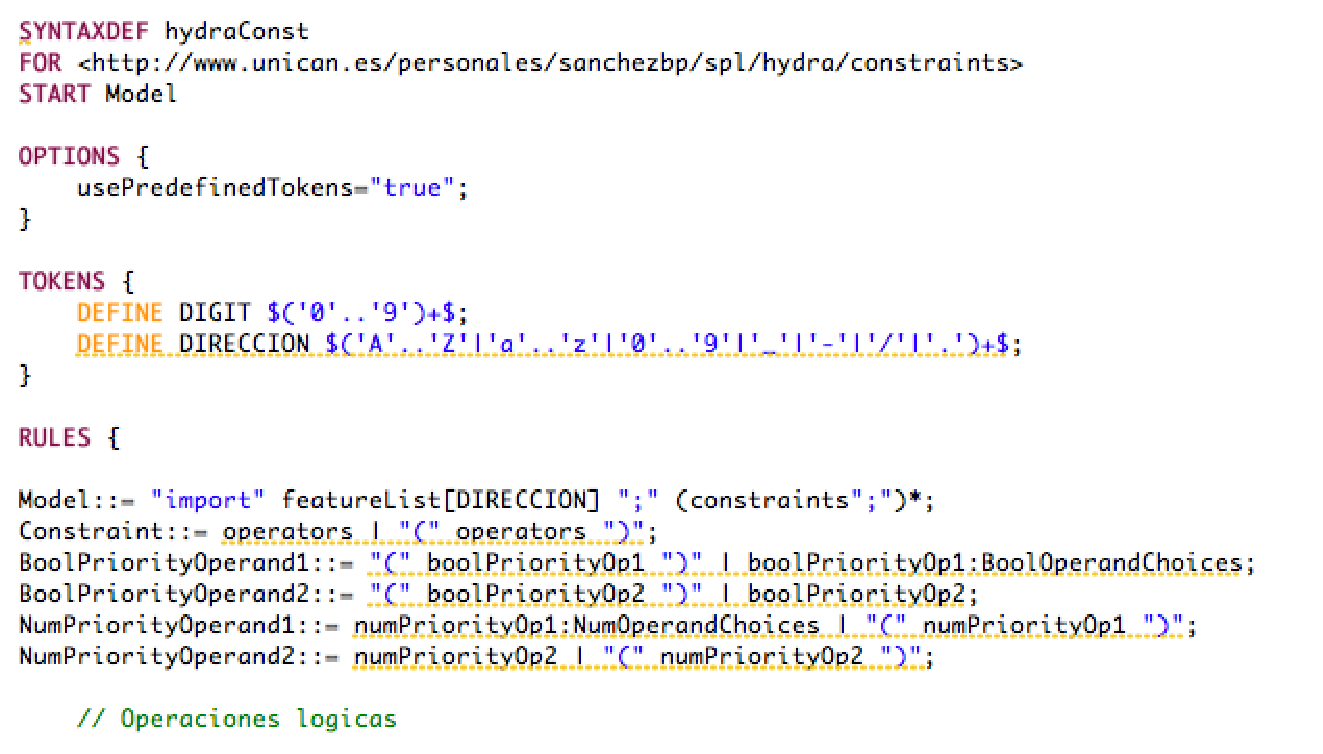
\includegraphics[scale=0.7]{gramatica/iniciogram.eps}
\caption{Implementaci�n del inicio de la gram�tica con EMFText. Con la figura \ref{figopers} se completa la gram�tica}
\label{figinitgram}
\end{figure}

Una vez comentados estos detalles es momento de explicar el inicio de la gram�tica, que se muestra en la figura \ref{figinitgram}. 

En la primera l�nea y mediante la cla�sula SYNTAXDEF indicamos la extensi�n que queremos que tengan los ficheros escritos en nuestro lenguaje. En nuestro caso nos hemos decantado por la terminaci�n .hydraConst. En la segunda l�nea y mediante la cla�sula FOR se indica la URI del metamodelo. Una URI es un formato de direcci�n interno de Eclipse, que se usa para localizar otros ficheros en el workspace. En la tercera l�nea, delimitada por la cla�sula START, indicamos a la gram�tica que la clase inicial de nuestro metamodelo (y la que ser� la raiz en todos los �rboles parseados) es Model.

El bloque OPTIONS permite activar algunas opciones de configuraci�n que incluye EMFText. En nuestro caso la �nica que tiene utilidad es usePredifinedTokens, que permite ahorrarnos la definici�n del token text. El bloque TOKENS sirve para definir los tokens de nuestra gram�tica. En nuestro caso usaremos 3: DIGIT para asignar al valor num�rico, TEXT para asignar a las caracter�sticas y DIRECCION para asignar la direcci�n f�sica del modelo de caracter�sticas.

Por �ltimo, el bloque RULES permite crear las producciones. Como inicial, tal y como se especific� en los requisitos, exigimos un import y una direcci�n, que ser� almacenada en el atributo featureList de la clase Model. En la l�nea inicial tambi�n se indica, mediante una expresi�n regular, que el n�mero de restricciones a definir puede ser tan grande como se desee y que estas deben acabar con el car�cter '';'' .

La l�nea de producci�n de Constraint diferencia entre operaciones con prioridad y sin ella. Sin el problema comentado de EMFText la gram�tica podr�a quedar as�, pero para solucionarlo nos vemos obligado a incluir las cuatro l�neas siguientes, cuya �nica funci�n es solventar esa situaci�n. El resto de la gram�tica continuar�a en la figura \ref{figopers} mostrada anteriormente, y ah� terminar�a.






\section{Pruebas}
\label{sec:gram:pruebas}
%%==========================================================================%%
%% Author : Abascal Fern�ndez, Patricia                                     %%
%% Author : S�nchez Barreiro, Pablo                                         %%
%% Version: 1.1, 15/05/2013                                                 %%
%%                                                                          %%
%% Memoria del Proyecto Fin de Carrera                                      %%
%% Application Engineering/Pruebas                                          %%
%%==========================================================================%%

Una vez implementados los generadores de c�digo para la fase de \emph{Ingenier�a de Aplicaciones}, el siguiente paso era dise�ar y ejecutar las pruebas necesarias que permitiesen comprobar el correcto funcionamiento de estos generadores. Para dise�ar las pruebas,  siguiendo el mismo procedimiento que en el caso anterior, utilizando la t�cnica de clases de equivalencia y valores l�mites, para luego completar con casos espec�ficos que permitiesen alcanzar el 100\% de la cobertura.  

A diferencia de la fase de \emph{Ingenier�a del Dominio}, en esta fase no se utiliz� \emph{EUnit} para ejecutar dichas pruebas, ya que dicha herramienta no se ajustaba a nuestras necesidades. Por tanto, se crearon los casos de prueba y se ejecutaron a mano, analizando de forma tambi�n manual si la salida producida coincid�a con la esperada. La Tabla~\ref{app:table:pruebas} muestra algunos de los casos de prueba ejecutados.

\begin{table}
\begin{small}
\begin{tabularx}{\linewidth}{|X|l|}
 \hline
{Casos v�lidos}&{Casos no v�lidos} \\ \hline
Configuraci�n con un solo camino hoja-raiz & Paquetes recursivos. \\
Configuraci�n con varios caminos y todos los m�todos independientes &\\
Configuraci�n con varios caminos y alg�n m�todo dependiente &\\
Configuraci�n con varios caminos, donde alg�n m�todo tiene versiones dependientes e independientes &\\
\hline
\end{tabularx}
\end{small}
\caption{Casos de prueba para la fase de Ingenier�a de la Aplicaci�n}
\label{app:table:pruebas}
\end{table}%

Una vez creados y probados los generadores de c�digo, el siguiente paso era empaquetarlos para posibilitar su distribuci�n y uso. La siguiente secci�n describe como se realiza dicha fase de despliegue.
Tras ejecutar estos casos de prueba y comprobar que los generadores de c�digo funcionaban correctamente, d�bamos por concluida la labore de desarrollo de los generadores de c�digo, restando solo su empaquetado y despliegue.


